182. \begin{figure}[ht!]
\center{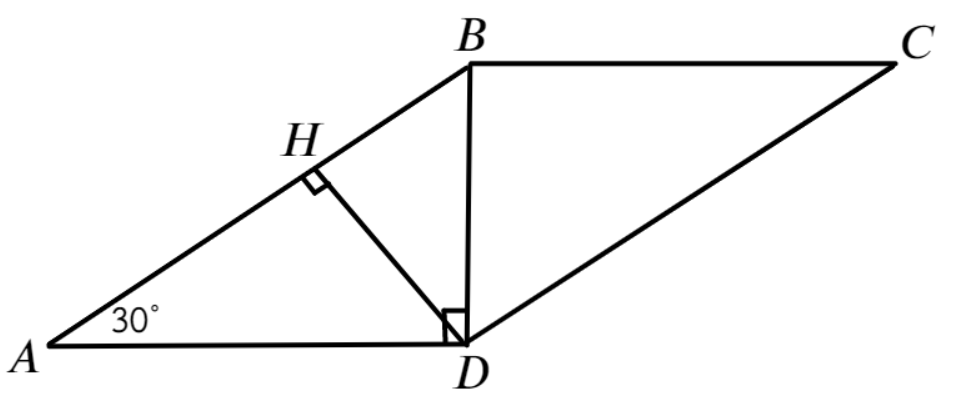
\includegraphics[scale=0.35]{g8-181.png}}
\end{figure}\\
В прямоугольном треугольнике $ABD$ катет $BD$ равен половине гипотенузы $AB,$ значит $\angle A=30^\circ.$ Прямые $AB$ и $CD$ параллельны, значит расстояние между ними равно длине любого перпендикуляра, опущенного из точки одной прямой на другую. Опустим перпендикуляр $DH$ из точки $D.$ В прямоугольном треугольнике $AHD$ угол $A$ равен $30^\circ,$ значит $DH=\cfrac{1}{2}AD=\cfrac{1}{2}BC=2.$\newpage\noindent
